\documentclass[]{article}
\usepackage{graphicx}
\usepackage{amsmath,amssymb,amsthm}
\usepackage{empheq}
\usepackage{float}
\usepackage[left=0.85in,top=0.85in,right=0.85in,bottom=0.85in]{geometry} % Document margins

% Title Page
\title{CS 6640 Project 4}
\author{Travis Allen, u1056595}


\begin{document}
	\maketitle
	
	\newpage
	\section{Preliminaries}

	\vskip 10pt

	\textbf{I chose to do project 4a: Image Mosaicing.} The code for this can be found in the \texttt{proj\_4.py} and \texttt{functions.py} files. \texttt{proj\_4.py} contains the actual algorithm developed to make a mosaic of greyscale images whose correspondences are documented in a \texttt{.json} file. \texttt{functions.py} contains some useful functions that would have otherwise crowded the \texttt{proj\_4.py} file. My solution to this project relies heavily on\texttt{numba}, so you must have that installed to run my code. I use it because it \emph{dramatically} speeds up the run time. 

\section{Experiments}	
	\subsection{Given Dataset}
	
	\newpage
	
	\subsection{Panoramic Images}
		I used the following panoramic images to see how the algorithm performs on them. I compared the results with 4 and 10 correspondence points.
	
	\begin{figure}[H]
		\centering
		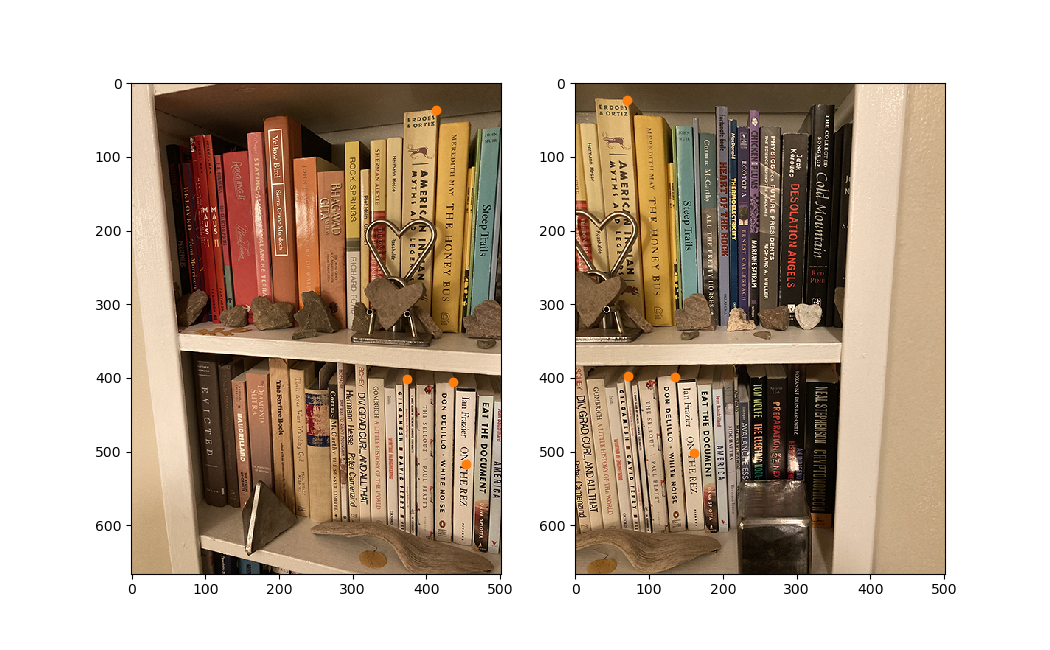
\includegraphics[width=6.5in]{test_images/shelf_4_correspondences.png}
		\caption{Bookshelf with 4 correspondences. I picked this image because it contains many corners, so accurately picking correspondences was straightforward.}
	\end{figure}
	
	\begin{figure}[H]
		\centering
		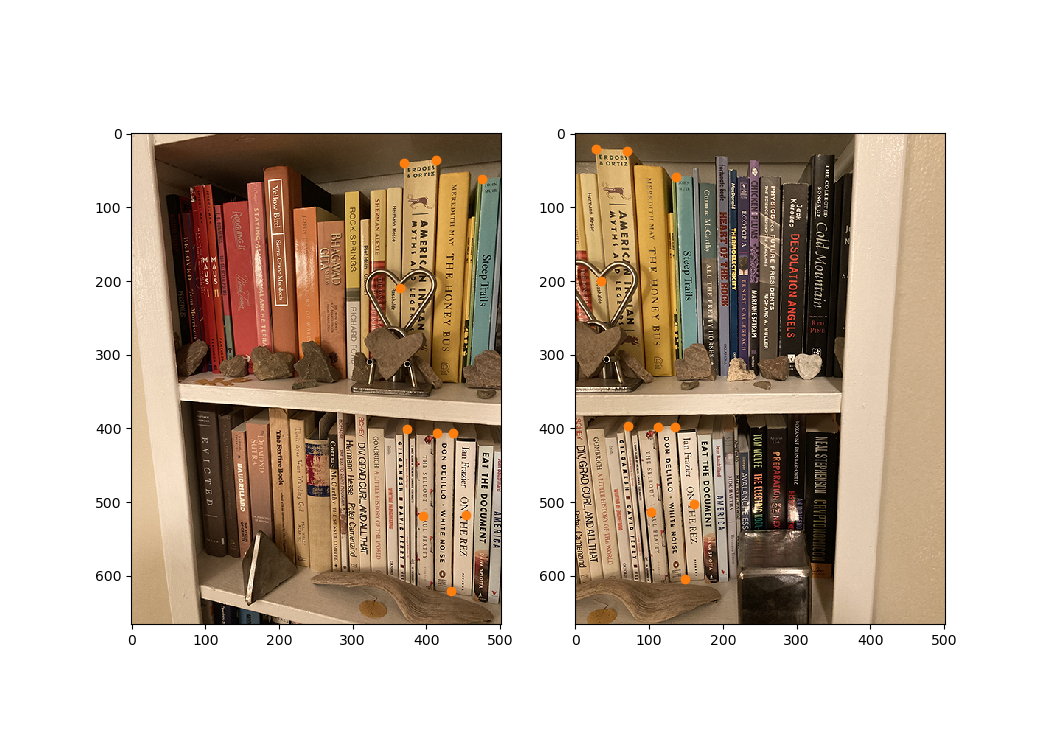
\includegraphics[width=6.5in]{test_images/shelf_10_correspondences.png}
		\caption{Bookshelf with 10 correspondences. I picked this image because it contains many corners, so accurately picking correspondences was straightforward.}
	\end{figure}

	\subsection{Planar Images}
		I used the following planar images to see how the algorithm performs on them. To construct them, I simply took a single image and cropped it twice to keep different, but overlapping parts of the image. Here I used 4 and 12 correspondence points, shown below.
		
		\begin{figure}[H]
			\centering
			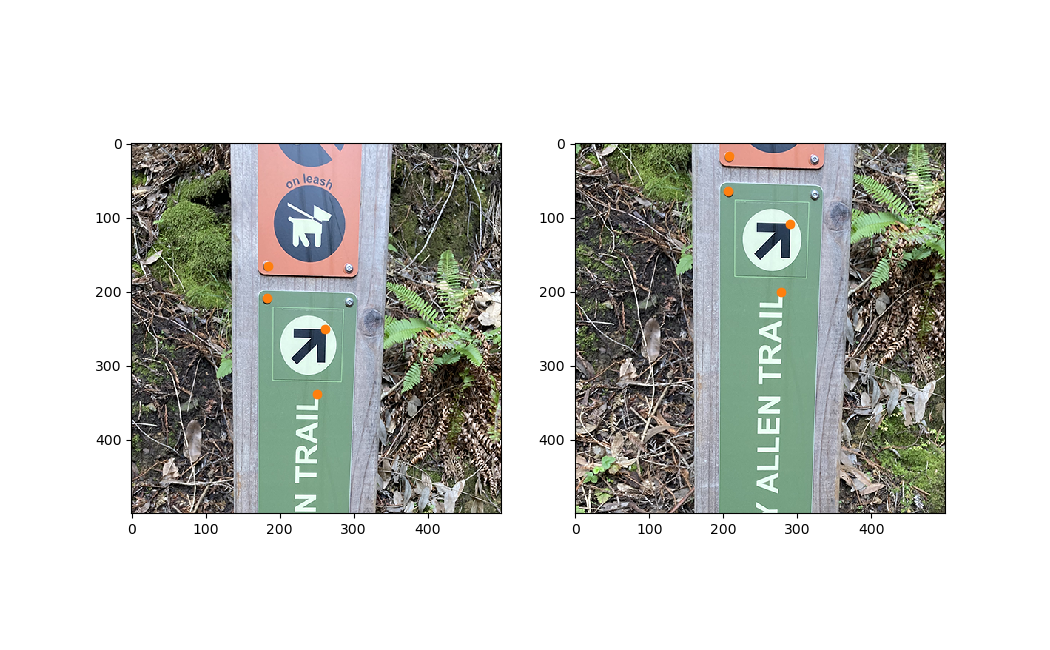
\includegraphics[width=6.5in]{test_images/sign_4_correspondences.png}
			\caption{Trail sign with 4 correspondences. I picked this image because it contains many corners, so accurately picking correspondences was straightforward.}
		\end{figure}
		
		\begin{figure}[H]
			\centering
			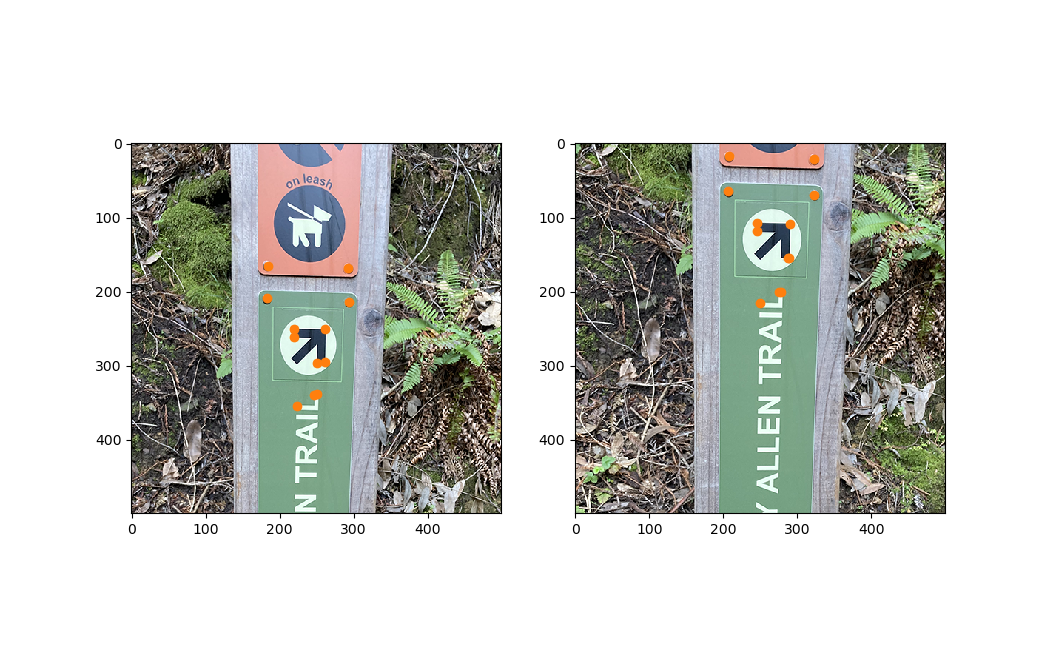
\includegraphics[width=6.5in]{test_images/sign_12_correspondences.png}
			\caption{Trail sign with 12 correspondences. I picked this image because it contains many corners, so accurately picking correspondences was straightforward.}
		\end{figure}
	
	\subsection{Number of Correspondences}
	\newpage
	
\section{Questions}
	\subsection{How many control points does it take to get a `good' transformation between images?}
	\subsection{How does the algorithm behave at the theoretical minimum of the number of control points?}
		The theoretical minimum number of correspondence points is 4 because that is the minimum possible number of points that allows the matrix below to have full rank. If this matrix has at least rank 8 and the number of rows is equal to the rank, then the system has an analytical solution. If the system has at least rank 8 and the number of rows is greater than the rank, then the system has a least-squares solution.
		\[\left(\begin{array}{cccccccc}
			-x_{1} & -y_{1} & -1 & 0 & 0 & 0 & x_{1} x_{1}^{\prime} & y_{1} x_{1}^{\prime} \\
			-x_{2} & -y_{2} & -1 & 0 & 0 & 0 & x_{2} x_{2}^{\prime} & y_{2} x_{2}^{\prime} \\
			-x_{3} & -y_{3} & -1 & 0 & 0 & 0 & x_{3} x_{3}^{\prime} & y_{3} x_{3}^{\prime} \\
			-x_{4} & -y_{4} & -1 & 0 & 0 & 0 & x_{4} x_{4}^{\prime} & y_{4} x_{4}^{\prime} \\
			0 & 0 & 0 & -x_{1} & -y_{1} & -1 & x_{1} y_{1}^{\prime} & y_{1} y_{1}^{\prime} \\
			0 & 0 & 0 & -x_{2} & -y_{2} & -1 & x_{2} y_{2}^{\prime} & y_{2} y_{2}^{\prime} \\
			0 & 0 & 0 & -x_{3} & -y_{3} & -1 & x_{3} y_{3}^{\prime} & y_{3} y_{3}^{\prime} \\
			0 & 0 & 0 & -x_{4} & -y_{4} & -1 & x_{4} y_{4}^{\prime} & y_{4} y_{4}^{\prime}
		\end{array}\right)\left(\begin{array}{c}
			p_{11} \\
			p_{12} \\
			p_{13} \\
			p_{21} \\
			p_{23} \\
			p_{23} \\
			p_{31} \\
			p_{32}
		\end{array}\right)=\left(\begin{array}{c}
			-x_{1}^{\prime} \\
			-x_{2}^{\prime} \\
			-x_{3}^{\prime} \\
			-x_{4}^{\prime} \\
			-y_{1}^{\prime} \\
			-y_{2}^{\prime} \\
			-y_{3}^{\prime} \\
			-y_{4}^{\prime}
		\end{array}\right)\]
		\begin{figure}[H]
			\centering
			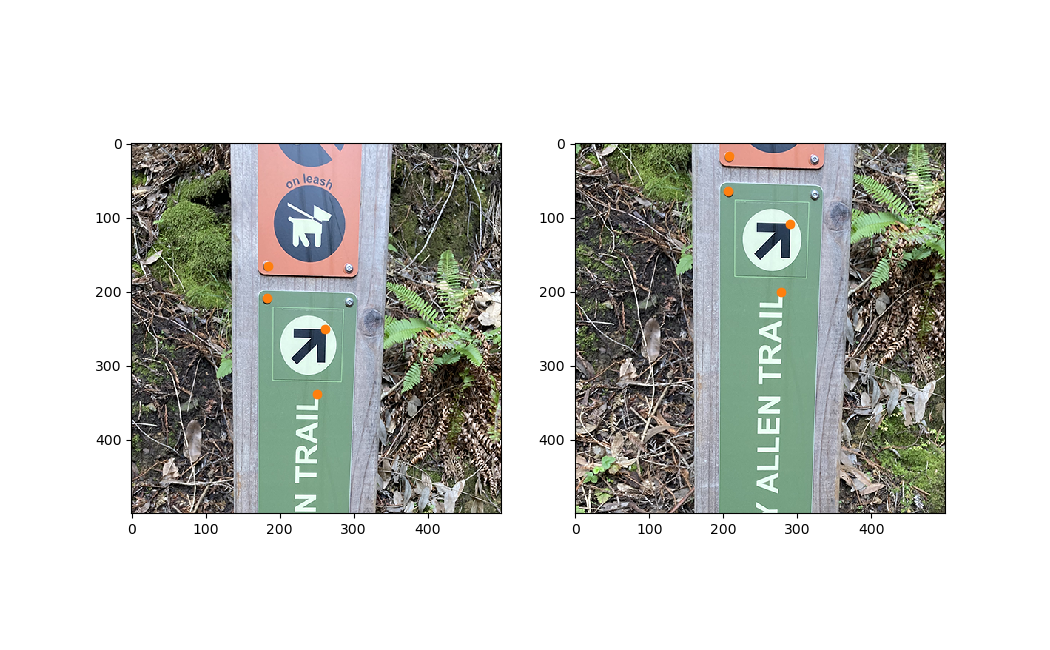
\includegraphics[width=6.5in]{test_images/sign_4_correspondences.png}
			\caption{Trail sign with 4 correspondences.}
		\end{figure}
		
		\begin{figure}[H]
			\centering
			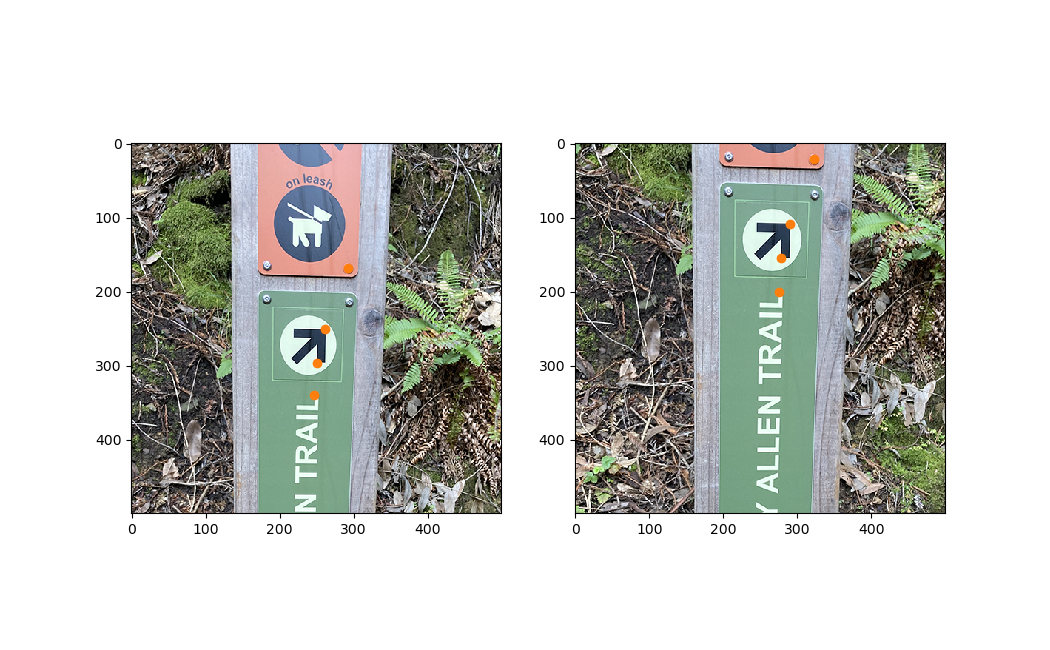
\includegraphics[width=6.5in]{test_images/sign_4_1_correspondences.png}
			\caption{Trail sign with 4 different correspondences.}
		\end{figure}
		
	\subsection{From your experiments, how does the accuracy of the control points affect the results?}

\section{Details}
	\subsection{Contrast}
	\subsection{Feathering}
	\subsection{Image Size}
	Initially, for $n$ number of images, I make a canvas that is $n+1$ times the size of the largest image so that I have enough room to work with when placing images in the mosaic. However, this often results in a canvas which is much larger than it needs to be. To return the canvas to a more reasonable size for viewing once the mosaic is complete, I execute the following procedure. I search through the large canvas to find the first and last rows and columns which contain only zero elements. I do this by using the \texttt{numpy.sum()} function on each row and column and checkign to see if it is equal to 0. The canvas consists of all zeros before I place images on it, so this method works by assuming that a row of all zeros contains no image information. I perform it this way because I figure that \texttt{numpy}'s vectorization is faster than my own implementation of computing the sum or individually inspecting every element in the image. 
	\begin{itemize}
	\item Place all of the images in a folder with a known path to the directory that contains \texttt{problem\_4.py}
	\item Place all of the names of all of the images in a \texttt{.txt} file in the folder, with each name separated by a new line
	\item Write the names of the folder and the file in lines \texttt{27} and \texttt{28} of \texttt{problem\_4.py}
	\item Write the maximum size of the images in lines \texttt{21} and \texttt{22} of \texttt{problem\_4.py}
	
\end{itemize}



\end{document}          

